\documentclass[10pt]{article}
\usepackage[utf8]{inputenc}
\usepackage{listings}
\usepackage[T1]{fontenc}
\usepackage{amsmath}
\usepackage{amsfonts}
\usepackage{amssymb}
\usepackage[version=4]{mhchem}
\usepackage{stmaryrd}
\usepackage{graphicx}
\usepackage[export]{adjustbox}
\graphicspath{ {./images/} }
\lstset{
    language=Python,
    basicstyle=\ttfamily,
    numbers=left,
    numberstyle=\tiny,
    frame=tb,
    columns=fullflexible,
    showstringspaces=false,
    breaklines=true,
    postbreak=\mbox{\textcolor{red}{$\hookrightarrow$}\space},
}

\title{Informe programación lineal }

\author{Diego de Santos del Río}
\date{18 de Septiembre, 2023}


\begin{document}
\maketitle
El problema que hay que resolver es el siguiente:\\
\\
Dado un escenario donde tienes un conjunto limitado de recursos y unidades disponibles, el objetivo es utilizar técnicas de programación lineal para maximizar el poder total de un ejército. Basándote en la información proporcionada:\\
\\
Recursos disponibles:\\
\\
Comida: 1200 | Madera: 800 | Oro: 600\\
\\
Unidades y sus costos:\\
\\
Espadachín: 60 de comida, 20 de madera, 0 de oro y 70 de poder.\\
Arquero: 80 de comida, 10 de madera, 40 de oro y 95 de poder.\\
Jinete: 140 de comida, 0 de madera, 100 de oro y 230 de poder.\\
\\
Primero voy a definir que tanto los espadachines, arqueros y jinetes son números positivos enteros, con lo que defino las siguientes ecuaciones:\\
\\
$$
\begin{gathered}
0 \leq \text { espadachines } \leq \infty \\
0 \leq \text { arqueros } \leq \infty \\
0 \leq \text { jinetes } \leq \infty
\end{gathered}
$$

Pero tenemos unas restricciones con los recursos que van a generar un problema el cual tenemos que resolver de la forma más óptima:

$$
\begin{aligned}
& 60 \times \text { espadachines }+80 \times \text { arqueros }+140 \times \text { jinetes } \leq 1200 \\
& 20 \times \text { espadachines }+10 \times \text { arqueros } \leq 800 \\
& 40 \times \text { arqueros }+100 \times \text { jinetes } \leq 600
\end{aligned}
$$

Expresando así las restricciones de comida, madera y oro respectivamente.

El objetivo es reclutar el ejército con mayor poder en función de la siguiente tabla:

\begin{center}
\begin{tabular}{|c|c|}
\hline
Ejército & Poder \\
\hline
Espadachín & 70 \\
\hline
Arquero & 95 \\
\hline
Jinete & 230 \\
\hline
\end{tabular}
\end{center}

Con esto obtenemos la siguiente ecuación:

$$
\text { Máx }(70 \times \text { espadachines }+95 \times \text {arqueros}+230 \times \text { jinetes })
$$

Implementando esto en nuestro código:

\begin{verbatim}
# Importo la librería ortools
from ortools.linear_solver import pywraplp
# Creo el solver
solver = pywraplp.Solver('Maximiza el poder del ejército',
                         pywraplp.Solver.GLOP_LINEAR_PROGRAMMING)

# Defino las variables con IntVar ya que son números enteros
espadachines = solver.IntVar(0, solver.infinity(), 'espadachines')
arqueros = solver.IntVar(0, solver.infinity(), 'arqueros')
jinetes = solver.IntVar(0, solver.infinity(), 'jinetes')

# Incluyo las restricciones
solver.Add(espadachines*60 + arqueros*80 + jinetes*140 <= 1200)  # Comida
solver.Add(espadachines*20 + arqueros*10 <= 800)                 # Madera
solver.Add(arqueros*40 + jinetes*100 <= 600)                     # Oro
# Máximizo la función objetivo
solver.Maximize(espadachines*70 + arqueros*95 + jinetes*230)
# Resuelvo el problema
status = solver.Solve()
# Imprimo la solución si es óptima
if status == pywraplp.Solver.OPTIMAL:
    print('================= Solución =================')
    print(
        f'Resuelto en {solver.wall_time():.2f} con {solver.iterations()} iteraciones.')
    print(f'Poder óptimo = {solver.Objective().Value()} poder')
    print('Army:')
    print(f'espadachines = {espadachines.solution_value()}')
    print(f'arqueros = {arqueros.solution_value()}')
    print(f'jinetes = {jinetes.solution_value()}')
else:
    print('El problema no tiene solución óptima.')
\end{verbatim}
\newpage
Obtenemos el siguiente resultado:\\
\\
\begin{center}
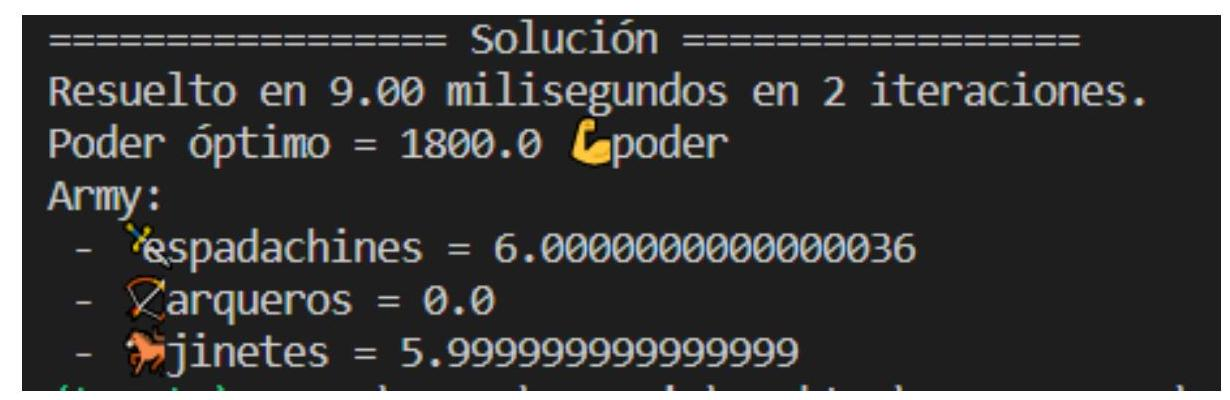
\includegraphics[max width=\textwidth]{images/solucion.jpg}
\end{center}

Por lo tanto, lo óptimo son 6 espadachines y 6 jinetes de forma que obtenemos el máximo de poder acorde a las restricciones impuestas.\\
\\
Es importante recalcar que he resuelto el problema utilizando el solucionador de problemas de optimización lineal de OR-Tools llamado GLOP (Paquete de optimización lineal de Google), el cual utiliza el método Simplex junto a técnicas avanzadas de optimización como el método de punto interior o método de la barrera para poder resolver este tipo de problemas


\end{document}
